\documentclass[10pt, conference, compsocconf]{llncs}
% Add the compsocconf option for Computer Society conferences.
%
% If IEEEtran.cls has not been installed into the LaTeX system files,
% manually specify the path to it like:
% \documentclass[conference]{../sty/IEEEtran}
\newcommand{\highlight}[1]{\colorbox{yellow}{#1}}




% Some very useful LaTeX packages include:
% (uncomment the ones you want to load)

% *** MISC UTILITY PACKAGES ***
%
%\usepackage{ifpdf}


% *** CITATION PACKAGES ***
%
%\usepackage{cite}


% *** MATH PACKAGES ***
%
%\usepackage[cmex10]{amsmath}

% *** SPECIALIZED LIST PACKAGES ***
%
%\usepackage{algorithmic}

% *** ALIGNMENT PACKAGES ***
%
%\usepackage{array}

% *** SUBFIGURE PACKAGES ***
\usepackage[tight,footnotesize]{subfigure}

% *** FLOAT PACKAGES ***
%
\usepackage{fixltx2e}

\usepackage{stfloats}

\usepackage{graphicx}

\usepackage{amsmath}
\usepackage{amssymb}

% *** LANGUAGE PACKAGES ***
%
\usepackage[utf8]{inputenc} 
\usepackage[T1]{fontenc}      
\usepackage[francais]{babel} 
\usepackage[top=4cm, bottom=4cm, left=4cm, right=4cm]{geometry}


\begin{document}
%
% paper title
% can use linebreaks \\ within to get better formatting as desired
\title{Le numérique dans\\l'accomplissement des SDGs}





% author names and affiliations
% use a multiple column layout for up to two different
% affiliations
% 
\author{Djavan Sergent \\
Master Sciences Informatiques \\
Phone: +41 78 602 77 48 \\
 \{djavan.sergent@etu.unige.ch\}}

\institute{Université de Genève}



% make the title area
\maketitle


\begin{abstract}
	<ABSTRACT>
\end{abstract}


\textbf{Keywords}
SDG; Citizen Science; Monitoring; Biodiversity;...;




\section{Introduction}\label{sec:introduction}

		En 2000, les Nations-Unies lancent le programme des Millenim Developpment Goals (MDGs) qui s'étend jusq'en 2015. Il s'agit d'un ensemble d'objectifs internationaux parmi lesquels on peut notamment citer l'éradication de l'extrême pauvreté et de la faim, combattre la mortalité infantile ou encore apporter une éducation à toutes et tous. Les 191 états membres des Nations-Unies ainsi que 22 organisations internationnales se sont engagées à participer activement à la réalisation de ces objectifs.
\begin{figure}
	\begin{center}
		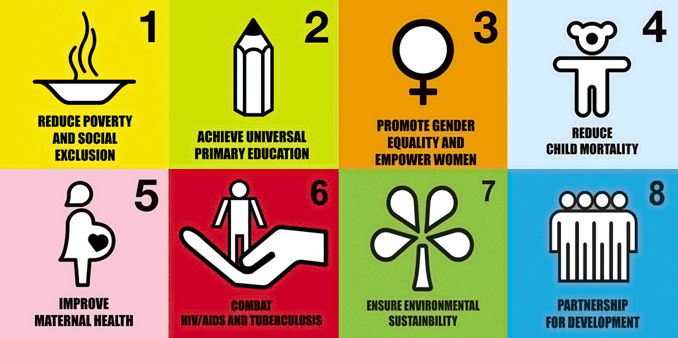
\includegraphics[width=200pt]{mdgs-full.png}
	\end{center}
	\caption{Représentation des MDGs}
\end{figure}

La situation en 2015 était que beaucoup d'efforts ont été investis, mais les progrès sont encore très inégaux. Les différents pays membres des Nations-Unies ainsi que des organisations civiles se sont donc intéressées à l'agenda post-2015, c'est à dire aux objectifs futurs. Les Sustainable Developpment Goals (SDGs) ont étés acceptés comme relève des MDGs. Ceux-ci comportent 17 buts, chacuns subdivisé en objectifs. Les SDGs totalisent 169 objectifs possédant chacuns leurs propres indicateurs.
\begin{figure}
	\begin{center}
		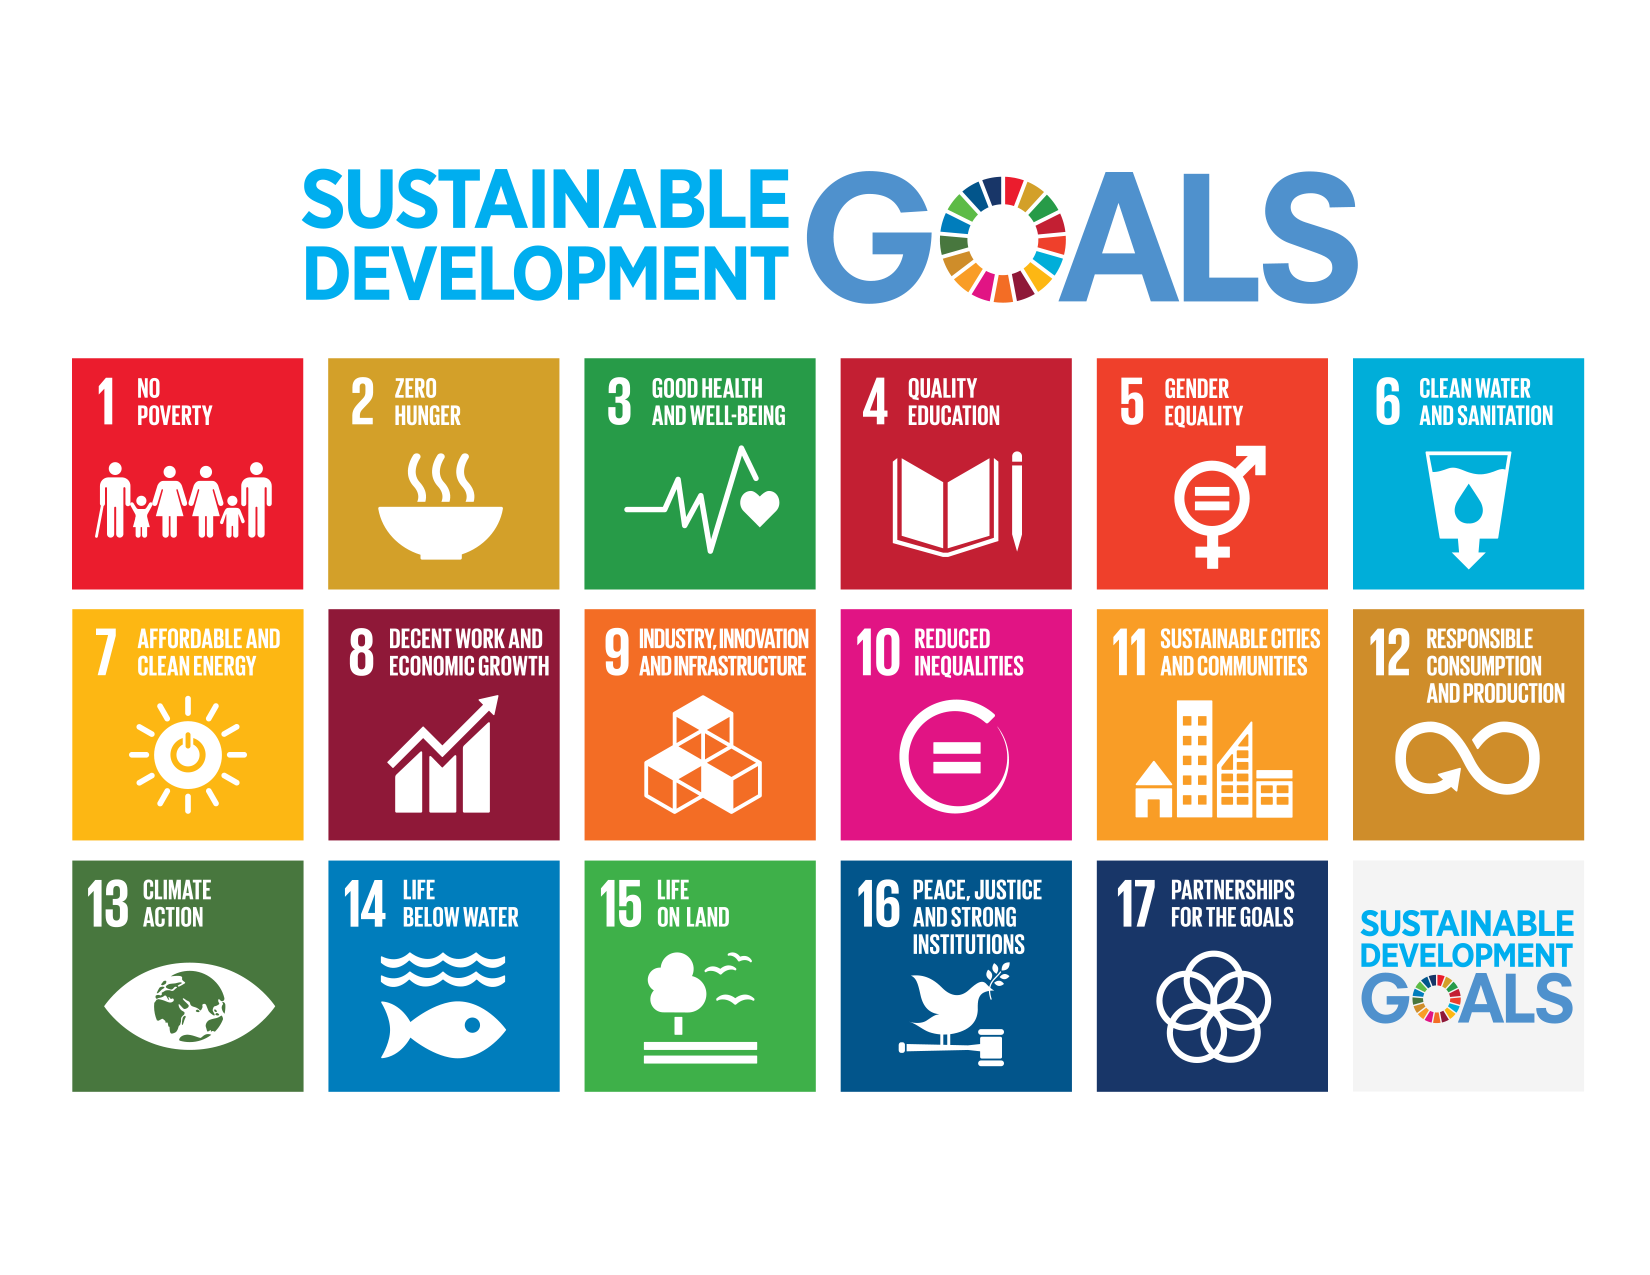
\includegraphics[width=200pt]{sdgs.jpg}
	\end{center}
	\caption{Représentation des SDGs}
\end{figure}

Nous analysons dans cet article le rôle du numérique dans la réalisation et le monitoring de certains de ces objectifs, particulièrement du point de vue de la participation citoyenne.

\subsection{Sustainable Developpment Goals}
\subsubsection{Objectifs}
Nous nous intéressons, dans le cadre de cet article, aux objectifs suivants :
\begin{description}
	\item[ 3 : Good-Health and Well-Being] Cet objectif se concentre sur les aspects qui concernent la santé, et en particulier la mortalité maternelle, natale et infantile, les maladies infectieuses, les morts prématurées, la polution de l'air, la sécurité et la mise en place de systèmes de soins et de financement.
	\item[ 6 : Clean water and sanitation] Les accès à l'eau et aux installations sanitaires sont essentiel pour la santé humaine, la prospérité économique et la préservation de l'environnement.  
	\item[13 : Climate Action] blabla
	\item[14 : Life below water] blabla
	\item[15 : Life on land] blabla
\end{description}


\subsubsection{Indicateurs}
Pour chaque objectif
\subsubsection{Progrès et revue}
\subsubsection{High-Level Political Forum}

\subsection{IT}


\section{Monitoring environnemental et sociétal}
\subsection{Indicateurs}
\subsubsection{Métriques}
\subsubsection{Définitions quantitatives}
\subsubsection{Impact environnemental}			
\subsubsection{Limites}

\subsection{Monitoring environnemental}
\subsubsection{Méthodes}
\subsubsection{Eau}
L'eau est une ressource extrêmement importante. Utilisée dans la vie de tous les jours par toutes et tous 
\subsubsection{Air}
\subsubsection{Territoire}
\subsubsection{Biodiversité}

\subsection{Monitoring sociétal}
\subsubsection{Santé}
\subsubsection{Sécurité}
\subsubsection{Développement}

\section{Participation citoyenne}
\subsection{Standards}
\subsection{Formation}
\subsection{Récupération de données}
\subsection{Traitement des données}
\subsection{Outils}
\subsubsection{Hardware}
\subsubsection{Software}
INatrualist, NatureBytes, Epicollect, SeeClickFix, Water Reporter, Project Noah	

\section{Projets}
\subsection{Aqueduct}
\subsection{InfoAmazonia}
\subsection{World Water Monitoring Day}
\subsection{Riverfly Monitoring Initiative}
\subsection{Restoration Assessment Initiative}
\subsection{Homebrew Sensing Project}
\subsection{Open Water Project}
\subsection{Open Air}
\subsection{Open Land}

\section{Conclusion}\label{sec:conclusion}
Summary of paper and future works.

% conference papers do not normally have an appendix


% use section* for acknowledgement
\section*{Acknowledgment}
The authors would like to thank...



\bibliographystyle{plain} %%% this is the style of the bibliograpyh
\bibliography{maindocument} %%% maindocument.bib is the file containing bibliographic entries


% that's all folks
\end{document}


